%=== CHAPTER FIVE (5) ===
%=== Discussion ===
\chapter{Fault Tolerance}
\begin{spacing}{1}
\setlength{\parskip}{0in}

\section{Design Ideas}

The UDP transport protocol is naively designed for low latency but not fault-tolerant transmission. UDP has no handshaking mechanism to guarantee reliable connections between clients and servers as compared to TCP. We implemented some techniques such as time-out, retransmit requests/responses, maintain histories and filter duplicated requests to guarantee the system to be fault-tolerant to message loss. 
Firstly, we design a three-way handshaking communication between servers and clients. When the server receives the response from clients, it processes the request and sends a response message piggybacking ACK to the client. At last, clients will send a ACK message to acknowledge whether it received the response successfully or not.\\

\begin{figure}[h!]
    \centering
  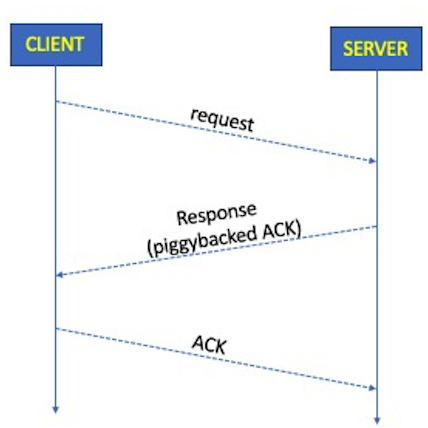
\includegraphics[width=6cm, height=6cm]{Image/4.png}
  \caption{Design}
\end{figure}

We considered three scenarios of message loss during transmission between server and client.
\subsection{Scenario 1: Request Loss}
This scenario is analyzed based on the assumption of Response and Acknowledgement are never lost.
As shown in Figure 4.2, to detect the request loss, we implemented a timeout mechanism on the client side. If a client doesn’t receive any replies from the server after a certain time, the client will send an acknowledgement message with status 0 (NAK). When the server receives a NAK message from the client, it will send a piggybacked NAK back to the client, So, the client will resend the request. This process keeps repeating until the client receives a piggybacked ACK message from the server.

\begin{figure}[h!]
\centering
  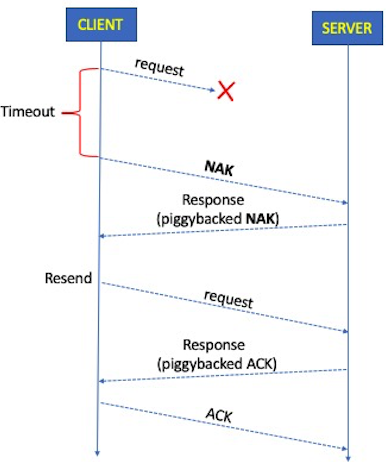
\includegraphics[width=6cm, height=6cm]{Image/2.png}
  \caption{Request Lost}
\end{figure}


\subsection{Scenario 2: Response Loss}
This scenario is analyzed based on the assumption of Request and Acknowledgement are never lost.
We also used the timeout mechanism on the client side to detect the response message loss during transmission. As shown in Figure 4.3, the differences with the scenario 1 is after the server (if enable At-Most-Once) receives a NAK message from client, the server will first get the message ID from the NAK message (more detailed in the Message Structure) , and then search in a maintained Hashtable with the messageID to check whether a previous processed request with the same message ID can be found.
If found, the server just resend the response message with piggybacking ACK. If not found, the server will just send a NAK back to the client (At-Least-Once just simply sends a NAK without searching in the Hashtable).


\begin{figure}[h!]
\centering
  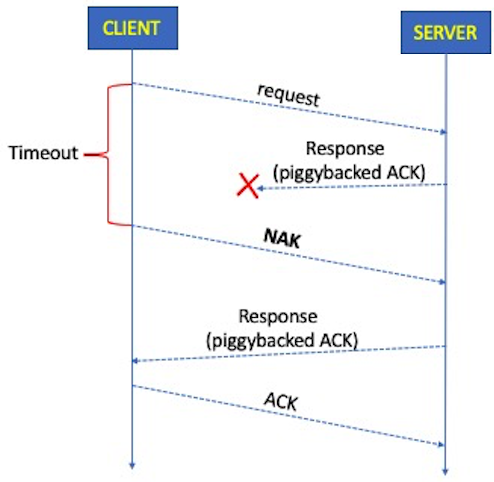
\includegraphics[width=6cm, height=6cm]{Image/1.png}
  \caption{Response Lost}
\end{figure}


\subsection{Senario 3: Acknowledgment Loss}
This scenario is analyzed based on the assumption of response and request are never lost. As shown in Figure 4.4, 
The purpose of the Acknowledgement is to acknowledge the client has successfully received the reply from the server or not. After receiving an ACK from client, server can remove the previous record in the Hashtable(if enable At-Most-Once). So, if the acknowledgment message is lost, the Hashtable storing previous processed records will never be removed. So, our proposed solution for this issue is to implement a timeout mechanism on the server side to auto remove a previous record within a certain time to avoid the Hashtable keeps growing. But, from the experience, the loss of an acknowledgement message won’t cause any operations to produce unexpected results.

\begin{figure}[h!]
\centering
  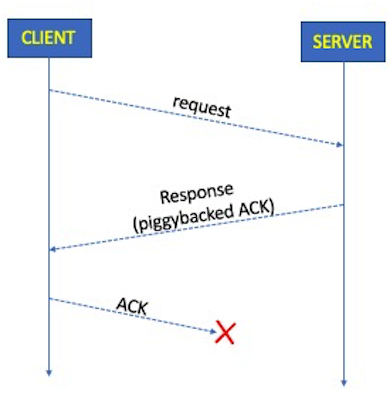
\includegraphics[width=6cm, height=5cm]{Image/3.png}
  \caption{Acknowledge Lost}
\end{figure}



\section{Experiments}

\subsection{Non-Idempotent}
We use our Service 5 (Auto-booking function) to conduct the three message lost scenarios with two different invocation semantics under the failure rate is 50\%. As shown in Table 4.1, we verified that the At-Least-Once semantics will invoke multiple times of bookings with randomly picking up the latest available slots on the server side under the response-loss scenario only.

\begin{table}[!h]
\centering
\begin{tabular}{|l|l|l|}
\hline
 & At-Least-Once & At-Most-Once \\ \hline
Request loss & \begin{tabular}[c]{@{}l@{}}Auto select one \\ latest available slots\end{tabular} & Auto select one latest available slots \\ \hline
Response loss & \begin{tabular}[c]{@{}l@{}}(\textbf{Unexpected})Auto select \\\textbf{multiple} latest available slots\end{tabular} & Auto select one latest available slots \\ \hline
Acknowledgement loss & \begin{tabular}[c]{@{}l@{}}Auto select one \\ latest available slots\end{tabular} & Auto select one latest available slots \\ \hline
\end{tabular}
\caption{Non-Idempotent}
\end{table}

\subsection{Idempotent}
We use our Service 6 (cancel bookings) to conduct the three message lost scenarios with two different invocation semantics under the failure rate is 50\%. As shown in Table 4.2, We verified that all the scenarios can produce correct operational results regarding of the invocation semantics.
\begin{table}[H]
\centering
\begin{tabular}{|l|l|l|}
\hline
 & At-Least-Once & At-Most-Once \\ \hline
Request loss & Booking is cancelled successfully & \begin{tabular}[c]{@{}l@{}} Booking is cancelled \\successfully\end{tabular} \\ \hline
Response loss &\begin{tabular}[c]{@{}l@{}} Booking is cancelled successfully(server)\\ (Booking ID is not found,client) \end{tabular} &\begin{tabular}[c]{@{}l@{}} Booking is cancelled \\successfully\end{tabular}  \\ \hline
Acknowledgement loss & Booking is cancelled successfully & \begin{tabular}[c]{@{}l@{}} Booking is cancelled \\successfully\end{tabular} \\ \hline
\end{tabular}
\caption{Idempotent}
\end{table}
\\

\chapter{Conclusion}
We designed and implemented a distributed booking system fault-tolerating to the message loss during transmission with UDP protocol.
We analysed and experimented three different message loss scenarios and implemented several mechanisms including timeout, re-transmit request/response messages, filter duplicated requests. Finally, we compared two different invocation semantics under three different message loss scenarios and found that the non-idempotent
operations could produce wrong results when applied At-Least-Once semantic under the response-loss scenario.

%=== END OF CHAPTER FIVE ===
\end{spacing}